\documentclass[../main/main.tex]{subfiles}

\newdate{date}{18}{11}{2020}

% \begin{figure}[h!]
% \centering
% \includegraphics[page=6,width=0.8\textwidth]{../lessons/pdf_file/18_lecture.pdf}
% \end{figure}

%\displaydate{date}. Compiled:  \today. Alice.

\begin{document}

\pagestyle{plain}

\section{Lecture 18}


\subsubsection*{Slide 1}

\begin{minipage}[]{0.5\linewidth}
\centering
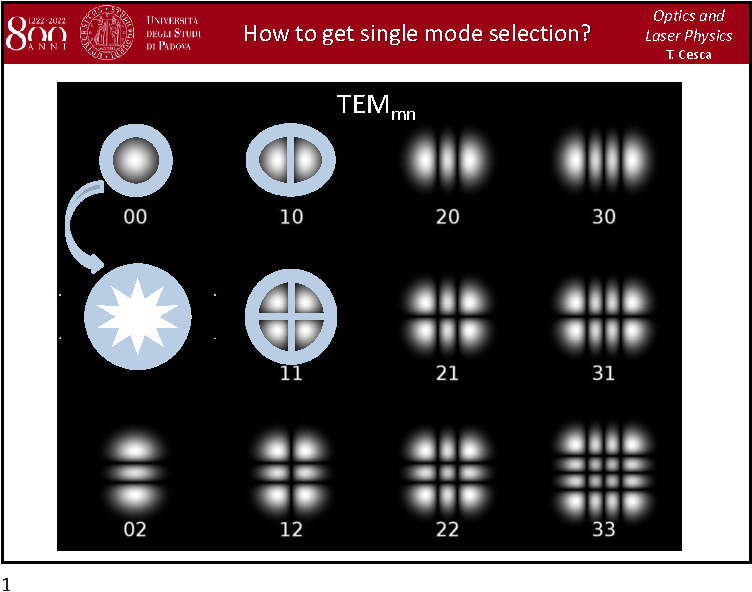
\includegraphics[page=1,width=1\textwidth]{../lessons/pdf_file/18_lecture.pdf}
\end{minipage}
\hspace{0.3cm}\vspace{0.3cm}
\begin{minipage}[c]{0.47\linewidth}

For mode locking we want multiple modes oscillating.

Instead, one of the working hypothesis for Q-switch and CW mode is to have one single mode oscillating in the cavity. How can we select one single mode?

For the transverse mode we have seen that the method to isolate modes is by using \textbf{diaframs}. The higher is the order of the mode that you want to isolate, the difficult is to construct a diagram which match the shape of the mode.

For transverse mode you typically isolate the TEM00 mode.

To conclude, a diafram induce high losses for all the mode which have a distribution in intensity different in space wrt to the mode you want to select.

\end{minipage}

\subsubsection*{Slide 2}

\begin{minipage}[]{0.5\linewidth}
\centering
\includegraphics[page=2,width=1\textwidth]{../lessons/pdf_file/18_lecture.pdf}
\end{minipage}
\hspace{0.3cm}\vspace{0.3cm}
\begin{minipage}[c]{0.47\linewidth}

For longitudinal mode selection the strategy is different.
Firstly, we need to talk about \textbf{thin-film interference}.

We have created a thin film of a material with \( n_2 \) on a substrate \( n_S \).

The two beam of reflection can interfere and create fringes of equal inclination. The phase shift between these two beams is \( \delta  \) (it is given by the path difference between these two rays). We should consider the possibility to have further contribution for reflection which depends on the relative refractive index.

\end{minipage}

\subsubsection*{Slide 3}

\begin{minipage}[]{0.5\linewidth}
\centering
\includegraphics[page=3,width=1\textwidth]{../lessons/pdf_file/18_lecture.pdf}
\end{minipage}
\hspace{0.3cm}\vspace{0.3cm}
\begin{minipage}[c]{0.47\linewidth}

The different of phase is \( k \Delta L \), where \( k \) is the wavevector in vacum.

\end{minipage}

\newpage

\subsubsection*{Slide 4}

\begin{minipage}[]{0.5\linewidth}
\centering
\includegraphics[page=4,width=1\textwidth]{../lessons/pdf_file/18_lecture.pdf}
\end{minipage}
\hspace{0.3cm}\vspace{0.3cm}
\begin{minipage}[c]{0.47\linewidth}

Since each interface produce a \( \pi  \) phase shift, we have no term of \( \Delta \Phi _{refl} \).
We want that \( \delta  \) is equal to \( 2 \pi  \) because we want to refllect most.


\end{minipage}

\subsubsection*{Slide 5}

\begin{minipage}[]{0.5\linewidth}
\centering
\includegraphics[page=5,width=1\textwidth]{../lessons/pdf_file/18_lecture.pdf}
\end{minipage}
\hspace{0.3cm}\vspace{0.3cm}
\begin{minipage}[c]{0.47\linewidth}


\end{minipage}

\subsubsection*{Slide 6}

\begin{minipage}[]{0.5\linewidth}
\centering
\includegraphics[page=6,width=1\textwidth]{../lessons/pdf_file/18_lecture.pdf}
\end{minipage}
\hspace{0.3cm}\vspace{0.3cm}
\begin{minipage}[c]{0.47\linewidth}

In the upper part of the film there is a black part. Before breaking the film can become very thin, the phase shift at this position has no contribution to the difference of path. The total phase shift is at this position equal to \( \pi  \): we have destructive interference, that is why we do not see any light in this point!

\end{minipage}

\newpage

\subsubsection*{Slide 7}

\begin{minipage}[]{0.5\linewidth}
\centering
\includegraphics[page=7,width=1\textwidth]{../lessons/pdf_file/18_lecture.pdf}
\end{minipage}
\hspace{0.3cm}\vspace{0.3cm}
\begin{minipage}[c]{0.47\linewidth}

Let us suppose that the slab is sufficiently large and we have to consider the interference not only between the first two beams but also the contribution of multiple beams. We want to see what happens.

\textbf{Any phase shift due to reflection is already present inside the reflection coefficient!}

\end{minipage}

\subsubsection*{Slide 8}

\begin{minipage}[]{0.5\linewidth}
\centering
\includegraphics[page=8,width=1\textwidth]{../lessons/pdf_file/18_lecture.pdf}
\end{minipage}
\hspace{0.3cm}\vspace{0.3cm}
\begin{minipage}[c]{0.47\linewidth}

Let us compute the field of the total transmitted beam.

\end{minipage}

\subsubsection*{Slide 9}

\begin{minipage}[]{0.5\linewidth}
\centering
\includegraphics[page=9,width=1\textwidth]{../lessons/pdf_file/18_lecture.pdf}
\end{minipage}
\hspace{0.3cm}\vspace{0.3cm}
\begin{minipage}[c]{0.47\linewidth}

We can do the same for the reflected beam.

\end{minipage}

\subsubsection*{Slide 10}

\begin{minipage}[]{0.5\linewidth}
\centering
\includegraphics[page=10,width=1\textwidth]{../lessons/pdf_file/18_lecture.pdf}
\end{minipage}
\hspace{0.3cm}\vspace{0.3cm}
\begin{minipage}[c]{0.47\linewidth}

Let us assume that \( n_1 = n_3 \) to simplify the problem.

Let us rewrite \( E_t \) and \( E_r \) as a function of the reflectance \( R \).

\end{minipage}

\subsubsection*{Slide 11}

\begin{minipage}[]{0.5\linewidth}
\centering
\includegraphics[page=11,width=1\textwidth]{../lessons/pdf_file/18_lecture.pdf}
\end{minipage}
\hspace{0.3cm}\vspace{0.3cm}
\begin{minipage}[c]{0.47\linewidth}

Now, let us consider the intensity.

This is the expression for the trasmitted intensity.

\end{minipage}

\subsubsection*{Slide 12}

\begin{minipage}[]{0.5\linewidth}
\centering
\includegraphics[page=12,width=1\textwidth]{../lessons/pdf_file/18_lecture.pdf}
\end{minipage}
\hspace{0.3cm}\vspace{0.3cm}
\begin{minipage}[c]{0.47\linewidth}

We can do the same for the reflected intensity.

\end{minipage}

\subsubsection*{Slide 13}

\begin{minipage}[]{0.5\linewidth}
\centering
\includegraphics[page=13,width=1\textwidth]{../lessons/pdf_file/18_lecture.pdf}
\end{minipage}
\hspace{0.3cm}\vspace{0.3cm}
\begin{minipage}[c]{0.47\linewidth}

Let us simploify these expressions by introducing the \textbf{coefficient of finesse} (of the slab of the material with refractive index \( n_2 \)).

These expressions are known as \textbf{Airy's formulas}.

\end{minipage}

\subsubsection*{Slide 14}

\begin{minipage}[]{0.5\linewidth}
\centering
\includegraphics[page=14,width=1\textwidth]{../lessons/pdf_file/18_lecture.pdf}
\end{minipage}
\hspace{0.3cm}\vspace{0.3cm}
\begin{minipage}[c]{0.47\linewidth}

If you shine a beam of light on a slab of material, in reflection you will get the minimum at certain position.. or if you want you have fringes in the intensity that is trasmitted or you have minima in the refreclted pattern.

If \( R \) is very large you have very narrow fringes in trasmission (or very narrow black lines in reflection), for small value of \( R \) they are definetely less defined and broadened.

\end{minipage}

\subsubsection*{Slide 15}

\begin{minipage}[]{0.5\linewidth}
\centering
\includegraphics[page=15,width=1\textwidth]{../lessons/pdf_file/18_lecture.pdf}
\end{minipage}
\hspace{0.3cm}\vspace{0.3cm}
\begin{minipage}[c]{0.47\linewidth}

This is an example for different value of \( R \) for the trasmitted intensity.

\end{minipage}

\subsubsection*{Slide 16}

\begin{minipage}[]{0.5\linewidth}
\centering
\includegraphics[page=16,width=1\textwidth]{../lessons/pdf_file/18_lecture.pdf}
\end{minipage}
\hspace{0.3cm}\vspace{0.3cm}
\begin{minipage}[c]{0.47\linewidth}

A useful parameter to evaluate the degree of definition of a fringe is its \textbf{full width at half maximum (FWHM)}.

If \( F \) is sufficiently large (so the reflectivity of the slab is large), we can approximate..

Another useful parameter is \( \mathcal{F} \) which is the \textbf{finesse (of the fringes)}.
It is the difference between the difference in phase among two consecutive fringes divided by the full width at half maximum \( \gamma   \).

\end{minipage}

\subsubsection*{Slide 17}

\begin{minipage}[]{0.5\linewidth}
\centering
\includegraphics[page=17,width=1\textwidth]{../lessons/pdf_file/18_lecture.pdf}
\end{minipage}
\hspace{0.3cm}\vspace{0.3cm}
\begin{minipage}[c]{0.47\linewidth}

To sum up. We have assumed \( n_1 = n_2 \).

\end{minipage}

\subsubsection*{Slide 18}

\begin{minipage}[]{0.5\linewidth}
\centering
\includegraphics[page=18,width=1\textwidth]{../lessons/pdf_file/18_lecture.pdf}
\end{minipage}
\hspace{0.3cm}\vspace{0.3cm}
\begin{minipage}[c]{0.47\linewidth}

This is called \textbf{Fabry-Perot etalon}. In a cavity of a laser we have a slab of air between two mirrors. In two dimension is called a Fabry-Perot etalon.

\end{minipage}

\subsubsection*{Slide 19}

\begin{minipage}[]{0.5\linewidth}
\centering
\includegraphics[page=19,width=1\textwidth]{../lessons/pdf_file/18_lecture.pdf}
\end{minipage}
\hspace{0.3cm}\vspace{0.3cm}
\begin{minipage}[c]{0.47\linewidth}

We can determine the \textbf{Fabry-Perot bandwidth}.

Another parameter is the \textbf{free specrral range}. It is the difference in frequency that correspond to a difference in phase of \( 2 \pi  \).

\end{minipage}

\subsubsection*{Slide 20}

\begin{minipage}[]{0.5\linewidth}
\centering
\includegraphics[page=20,width=1\textwidth]{../lessons/pdf_file/18_lecture.pdf}
\end{minipage}
\hspace{0.3cm}\vspace{0.3cm}
\begin{minipage}[c]{0.47\linewidth}

We call it etalon any time the slab as a given and fixed thickness. You can also realize in this way \textbf{Fabry-Perot interferometer} if instead of having fixed thickness for the slab you can vary it. Or for instance we are able to move one of the two mirrors (the thick of the slab hence is varying).

\end{minipage}

\subsubsection*{Slide 21}

\begin{minipage}[]{0.5\linewidth}
\centering
\includegraphics[page=21,width=1\textwidth]{../lessons/pdf_file/18_lecture.pdf}
\end{minipage}
\hspace{0.3cm}\vspace{0.3cm}
\begin{minipage}[c]{0.47\linewidth}

The blue spectrum of emission is from an unknown material. Let us suppose that it passes trough a Fabry-Perot.

If we can move a mirror we can vary the position of the peak. So we can scan the material.

\end{minipage}

\subsubsection*{Slide 22}

\begin{minipage}[]{0.5\linewidth}
\centering
\includegraphics[page=22,width=1\textwidth]{../lessons/pdf_file/18_lecture.pdf}
\end{minipage}
\hspace{0.3cm}\vspace{0.3cm}
\begin{minipage}[c]{0.47\linewidth}

\end{minipage}

\subsubsection*{Slide 23}

\begin{minipage}[]{0.5\linewidth}
\centering
\includegraphics[page=23,width=1\textwidth]{../lessons/pdf_file/18_lecture.pdf}
\end{minipage}
\hspace{0.3cm}\vspace{0.3cm}
\begin{minipage}[c]{0.47\linewidth}

\end{minipage}

\subsubsection*{Slide 24}

\begin{minipage}[]{0.5\linewidth}
\centering
\includegraphics[page=24,width=1\textwidth]{../lessons/pdf_file/18_lecture.pdf}
\end{minipage}
\hspace{0.3cm}\vspace{0.3cm}
\begin{minipage}[c]{0.47\linewidth}

\textbf{How to use all of these in order to get longitudinal modes selection?}

It is possible to use a Fabry-Perot etalon to select. We have to satisfy this condition for the separation in frequency to have just one longitudinal mode that is amplified by the active medium. This condition become a condition in term of the effective length.

Let us try to make some calculation.
We see that we should use too small effect length for the active medium. That is why we use Fabry-Perot etalon to solve the problem.

\end{minipage}

\subsubsection*{Slide 25}

\begin{minipage}[]{0.5\linewidth}
\centering
\includegraphics[page=25,width=1\textwidth]{../lessons/pdf_file/18_lecture.pdf}
\end{minipage}
\hspace{0.3cm}\vspace{0.3cm}
\begin{minipage}[c]{0.47\linewidth}

We have a material with a gain curve and we insert in the cavity a Fabry-Perot etalon. Now, the condition to satisfy to have one single mode is this one.
The second condition is that we want just one peak.


\end{minipage}

\subsubsection*{Slide 26}

\begin{minipage}[]{0.5\linewidth}
\centering
\includegraphics[page=26,width=1\textwidth]{../lessons/pdf_file/18_lecture.pdf}
\end{minipage}
\hspace{0.3cm}\vspace{0.3cm}
\begin{minipage}[c]{0.47\linewidth}

We obtain a condition for the effective length.

\end{minipage}

\subsubsection*{Slide 27}

\begin{minipage}[]{0.5\linewidth}
\centering
\includegraphics[page=27,width=1\textwidth]{../lessons/pdf_file/18_lecture.pdf}
\end{minipage}
\hspace{0.3cm}\vspace{0.3cm}
\begin{minipage}[c]{0.47\linewidth}

Let us see some examples.

\end{minipage}

\subsubsection*{Slide 28}

\begin{minipage}[]{0.5\linewidth}
\centering
\includegraphics[page=28,width=1\textwidth]{../lessons/pdf_file/18_lecture.pdf}
\end{minipage}
\hspace{0.3cm}\vspace{0.3cm}
\begin{minipage}[c]{0.47\linewidth}

If just one Fabry-Perot etalon is not enough, we can use two or even more Fabry-Perot etalon.

Let us see what happens when we use 2 Fabry-Perot etalon with same finesse and different thickness.

The thickest etalon (the largest) is used to discriminate two adjiacent longitudinal modes since it has a smaller bandwidth.

The thinnest etalon is used to have only one peak of the first etalon within the trasmittance peak of the second etalon.


\end{minipage}

\subsubsection*{Slide 29}

\begin{minipage}[]{0.5\linewidth}
\centering
\includegraphics[page=29,width=1\textwidth]{../lessons/pdf_file/18_lecture.pdf}
\includegraphics[page=30,width=1\textwidth]{../lessons/pdf_file/18_lecture.pdf}
\end{minipage}
\hspace{0.3cm}\vspace{0.3cm}
\begin{minipage}[c]{0.47\linewidth}

So we have three condition!

In this case we can increase a lot the effective length of the cavity.

The interference filter are the Fabry-Perot etalon.

\end{minipage}



\end{document}
